% -*- TeX:de -*-
\NeedsTeXFormat{LaTeX2e}
\documentclass[12pt,a4paper]{article}
\usepackage[german]{babel} % german text
\usepackage[DIV12]{typearea} % size of printable area
\usepackage[T1]{fontenc} % font encoding
%\usepackage[latin1]{inputenc} % most likely on Windows
\usepackage[utf8]{inputenc} % probably on Linux
\usepackage{multicol}

% PLOTTING
\usepackage{pgfplots} 
\usepackage{pgfplotstable}
\usepackage{url}
\usepackage{graphicx} % to include images
\usepackage{tikz}
\usepackage{subfigure} % for creating subfigures
\usepackage{amsmath} % a bunch of symbols
\usepackage{amssymb} % even more symbols
\usepackage{booktabs} % pretty tables
\usepackage{makecell} % multi row table heading

% a floating environment for circuits
\usepackage{float}
\usepackage{caption}

%\newfloat{circuit}{tbph}{circuits}
%\floatname{circuit}{Schaltplan}

% a floating environment for diagrams
%\newfloat{diagram}{tbph}{diagrams}
%\floatname{diagram}{Diagramm}

\selectlanguage{german} % use german

\begin{document}

%%%%%%% DECKBLATT %%%%%%%
\thispagestyle{empty}
			\begin{center}
			\Large{Fakultät für Physik}\\
			\end{center}
\begin{verbatim}


\end{verbatim}
							%Eintrag des Wintersemesters
			\begin{center}
			\textbf{\LARGE SS 14}
			\end{center}
\begin{verbatim}


\end{verbatim}
			\begin{center}
			\textbf{\LARGE{Physikalisches Praktikum\\ für das Bachelorstudium}}
			\end{center}
\begin{verbatim}




\end{verbatim}

			\begin{center}
			\textbf{\LARGE{PROTOKOLL}}
			\end{center}
			
\begin{verbatim}

\end{verbatim}

			\begin{flushleft}
			\textbf{\Large{Experiment (Nr., Titel): PS10 - Wärmeleitung in Metallen und Isolatoren, Spezifische Wärmekapazität von Metallen}}\\
							%Experiment Nr. und Titel statt den Punkten eintragen
			\LARGE{PS09 }	
			\end{flushleft}

\begin{verbatim}

\end{verbatim}	
							%Eintragen des Abgabedatums, oder des Erstelldatums des Protokolls
			\begin{flushleft}
			\textbf{\Large{Datum:}} \Large{08.05.2014}
			\end{flushleft}
			
\begin{verbatim}
\end{verbatim}
							%Namen der Protokollschreiber
		\begin{flushleft}
			\textbf{\Large{Namen:}} \Large{Patrick Braun, Johannes Kurz}
			\end{flushleft}

\begin{verbatim}


\end{verbatim}
							%Kurstag und Gruppennummer, zb. Fr/5
			\begin{flushleft}
			\textbf{\Large{Kurstag/Gruppe:}} \Large{DO/4}
			\end{flushleft}

\begin{verbatim}

\end{verbatim}
							%Name des Betreuers, das Praktikum betreute.
			\begin{flushleft}
			\LARGE{\textbf{Betreuer:}}	\Large{Johanna Akbarzadeh}	
			\end{flushleft}

%%%%%%% DECKBLATT ENDE %%%%%%%
\pagebreak
\setlength{\columnsep}{20pt}
\begin{multicols}{2}

%%%%%%%%%%%%%%%%%%%%%%%%%%%%%%%%%%%%%%%%%%%%%%%%

%\begin{figure}[H]
%	\centering
%	\includegraphics[scale=0.35]{./data/beugung.png}
%	\caption{Beugungsmuster Einzelspalt (echtes Foto; schwarz durch weiß ersetzt)}
%	\label{fig:beugungsmuster}
%\end{figure}


%\begin{figure}[H]
%	\centering
%	\pgfplotstabletypeset[
%			columns={abstand, n},
%			col sep=&,
%			columns/abstand/.style={precision=2, zerofill, column name=\makecell{$Abstand$\\$(\pm 0.05)[mm]$} }, 
%			columns/n/.style={column name=\makecell{$n$\\$(Ordnung)$}, precision=0},
%			every head row/.style={before row=\hline,after row=\hline\hline},
%			every last row/.style={after row=\hline},
%			every first column/.style={column type/.add={|}{} },
%			every last column/.style={column type/.add={}{|} }
%			]{
%			abstand & n
%			12.9 & 1
%			24.45 & 2
%			37.40 & 3
%			49.35& 4
%			62.45 & 5
%			74.45 & 6
%			87.45 & 7
%			100.25 & 8
%			
%			}
%	\caption{Messwerte Einzelspalt}
%	\label{tab:werte_einzelspalt}
%\end{figure}


%%%%%%%%%%%%%%%%%%%%%%%%%%%%%%%%%%%%%%%%%%%%%%%%
%%%%%%%%%%%%%%%%%%%%%%%%%%%%%%%%%%%%%%%%%%%%%%%%
\noindent In den folgenden Experimenten bestimmen wir die Transporteigenschaften von Festkörpern in Bezug auf Wärme. Kennzahlen die sich im laufe der Geschichte heraus kristallisiert haben sind:\\
\begin{itemize}
	\item Temperaturleitfähigkeit
	\item Wärmeleitfähigkeit
\end{itemize}
Diese geben an wie gut (oder schlecht bei Isolatoren) Temperaturen und somit Wärme im Festkörper propagiert werden.

\section{Wärmeleitfähigkeit von Metallen - thermografische Bestimmung}

\subsection{Grundlagen}
$$T(x,t) = (T_0 - T_{max}) * erf(\frac{1}{sqrt(4 * \chi * t)})+T_{max}$$
$$\chi = \frac{\lambda}{\rho*c}$$
$$\phi = const.$$
$$\frac{\delta Q}{\deltat} = -\lambda * A * \frac{dT}{dx}$$
\subsection{Versuchsaufbau}
Der erste Versuch gliedert sich in zwei Teilgebiete. Im ersten Teilgebiet betrachten wir zwei Metallstäbe (Eisen, lackiert). Einer der beiden wird auf 40 Grad erwärmt und der andere verbleibt bei Raumtemperatur. Mit ein wenig Wärmeleitpaste werden beide Stäbe zusammengefügt und mit der Wärmebildkamera (Abb. \ref{}) nach 30 und nach 60 Sekunden ein Bild erstellt.\\
Mit der Software Talios zur Auswertung der Infrarotbilder kann in einer Linie der Temperaturverlauf festgestellt werden.


\subsection{Resultate}

\begin{figure}[H]
	\centering
	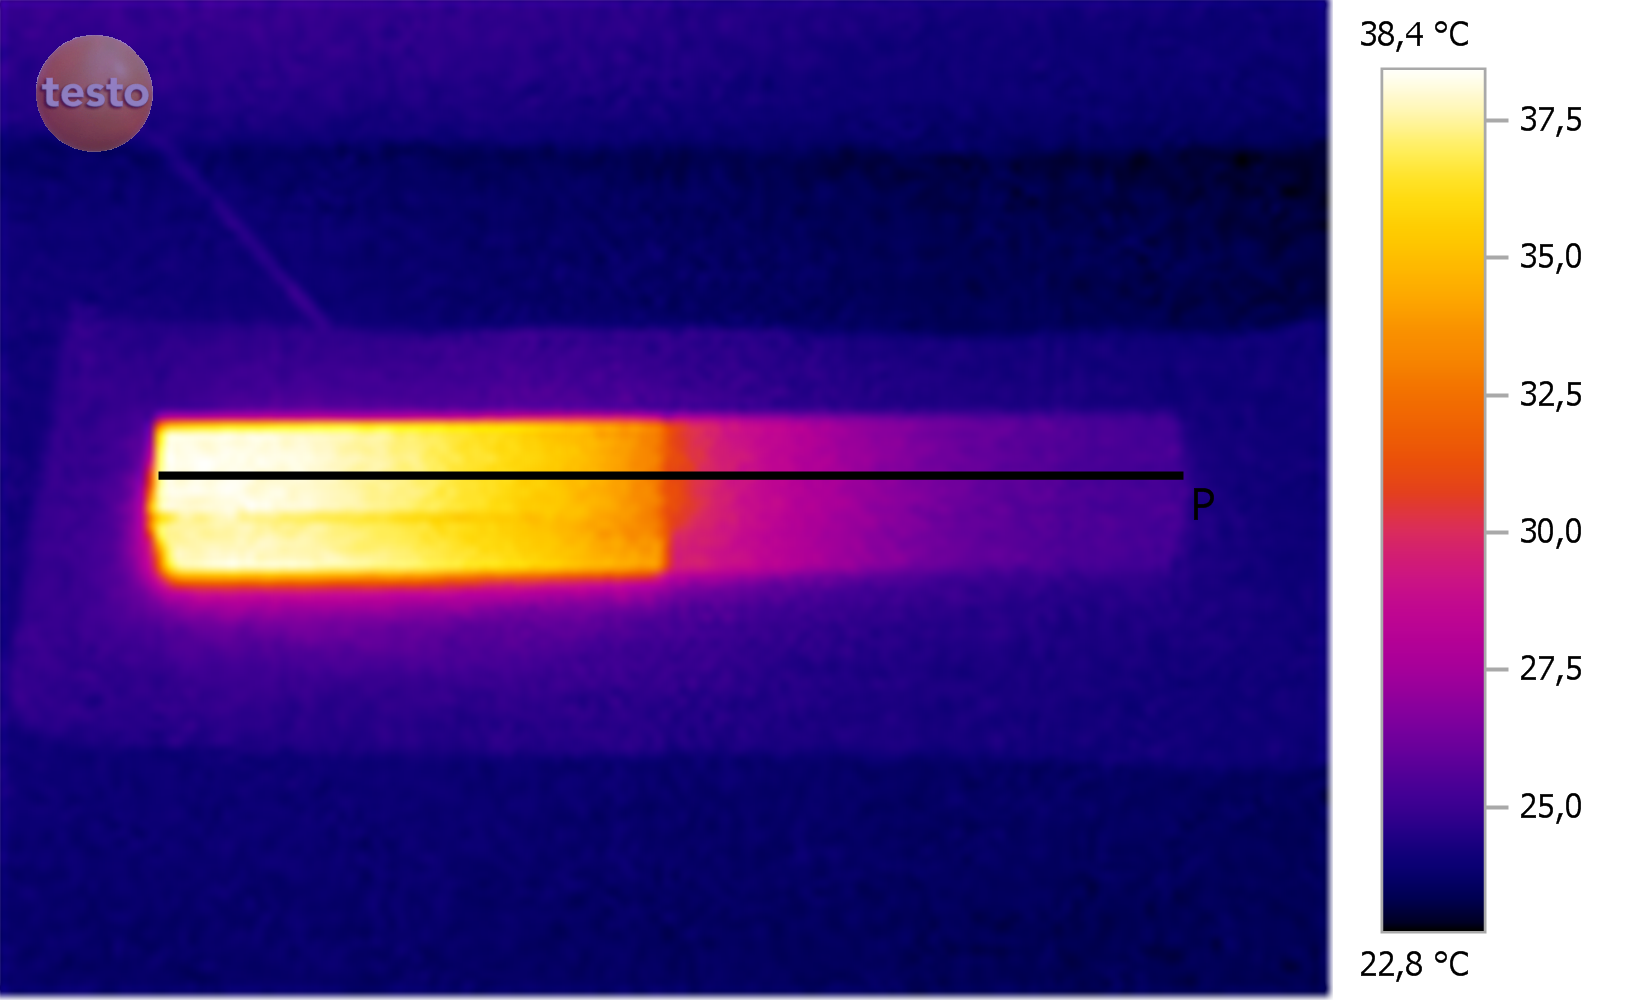
\includegraphics[scale=0.12]{./BilderCorrect/Versuch_1_gradient_60.png}
	\caption{Nicht stationärer Temperaturverlauf in Eisen}
	\label{fig:nicht_stat_verlauf}
\end{figure}

\begin{figure}[H]
	\centering
	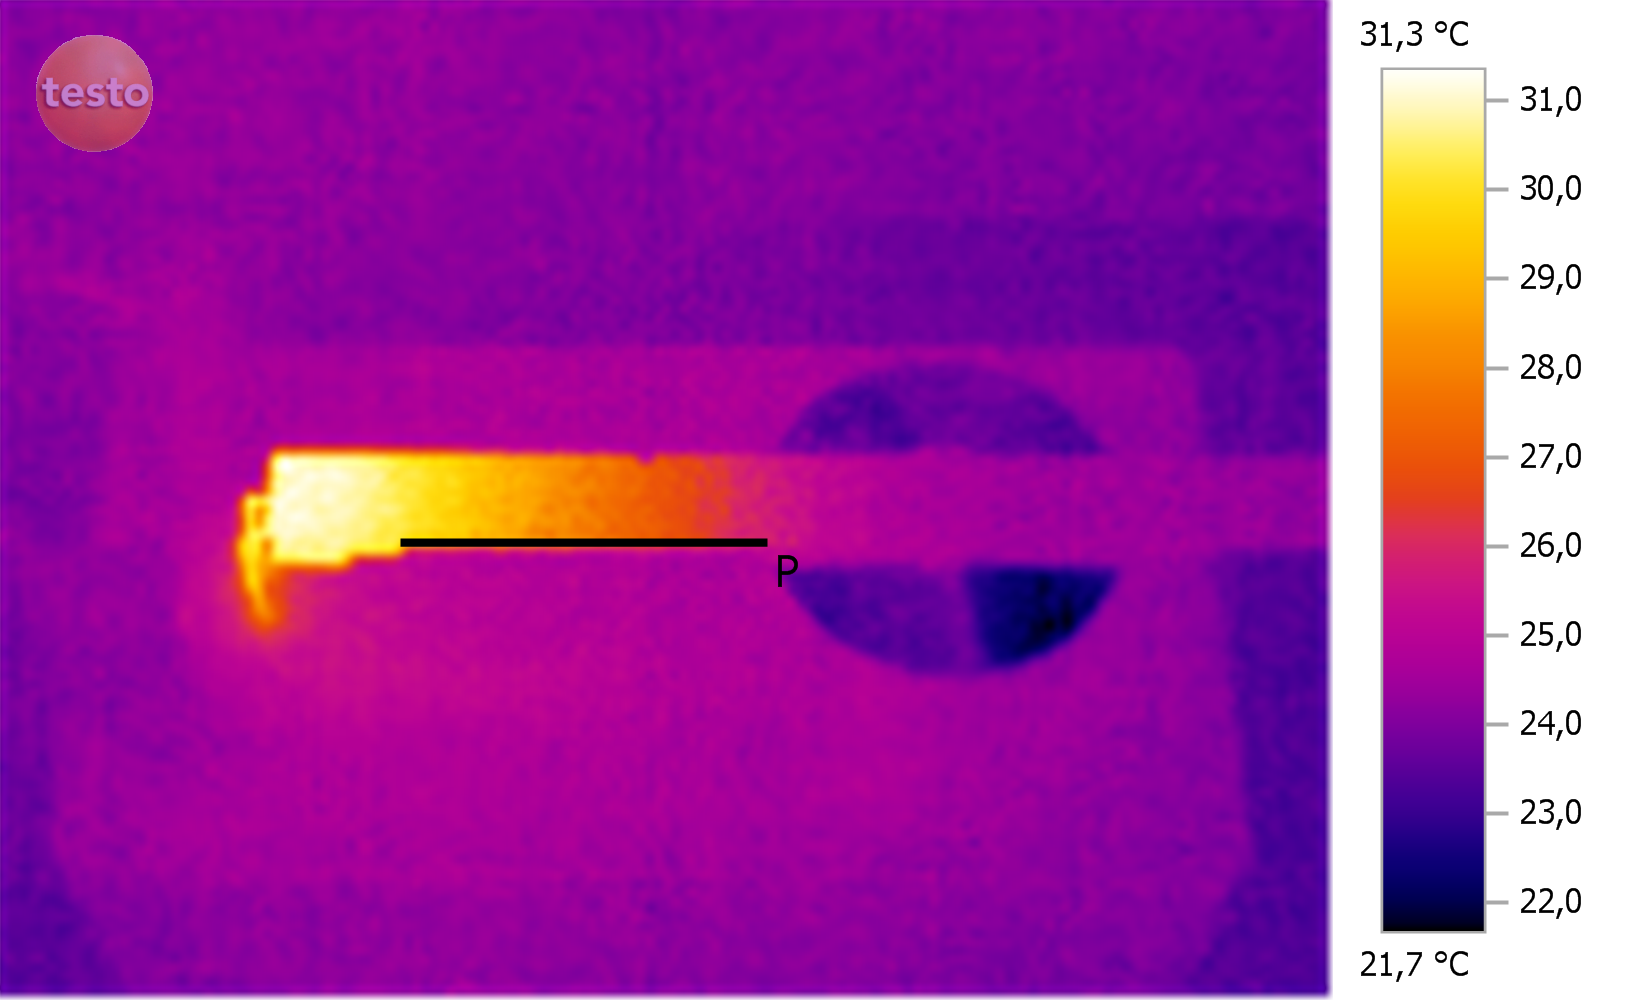
\includegraphics[scale=0.12]{./BilderCorrect/Versuch_1_stationaer_roh.png}
	\caption{Stationärer Temperaturverlauf in Aluminium}
	\label{fig:stat_verlauf}
\end{figure}



\begin{figure}[H]
	\centering
	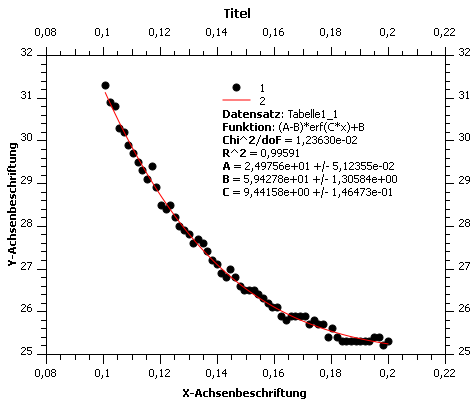
\includegraphics[scale=3.7]{./BilderCorrect/nicht_stationaer_temp_verlauf.png}
	\caption{Nicht stationärer Temperaturverlauf in Aluminium }
	\label{fig:stat_verlauf}
\end{figure}

\subsection{Diskussion}
Ein nicht klar hervorgegangener Sachverhalt der eine ordentliche Auswertung erst möglich macht, ist das die Wärmeleitpaste nur zur Verminderung des Luftpolsters zwischen den Stäben dient. Beim ersten Versuchsdurchlauf wurde zu viel Paste verwendet und daher ein steiler Temperaturabfall festgestellt (Isolator Wirkung).\\


%%%%%%%%%%%%%%%%%%%%%%%%%%%%%%%%%%%%%%%%%%%%%%%%
%%%%%%%%%%%%%%%%%%%%%%%%%%%%%%%%%%%%%%%%%%%%%%%%
\section{Wärmeleitfähigkeit von Wärmeisolatoren}

\subsection{Grundlagen}

\subsection{Versuchsaufbau}

\subsection{Resultate}

\subsection{Diskussion}


\section{Quellen}
$[1]$ Anleitung, \url{http://www.univie.ac.at/anfpra/neu1/ps/ps10/PS10.pdf}\\

\end{multicols}
\end{document}